\section{Testbed and Methodology}
\label{sec:method}

Fig.~\ref{fig:pipeline} shows the pipeline in the order the campaign ran it. The first steps
built the dependency graphs and the predictors and locked the analysis plan before any
campaign data existed. The middle steps repeated in every run, and the last ones ran once the
campaign was complete. Each box names the repository files that carry out the step.

\begin{figure}[!t]
\centering
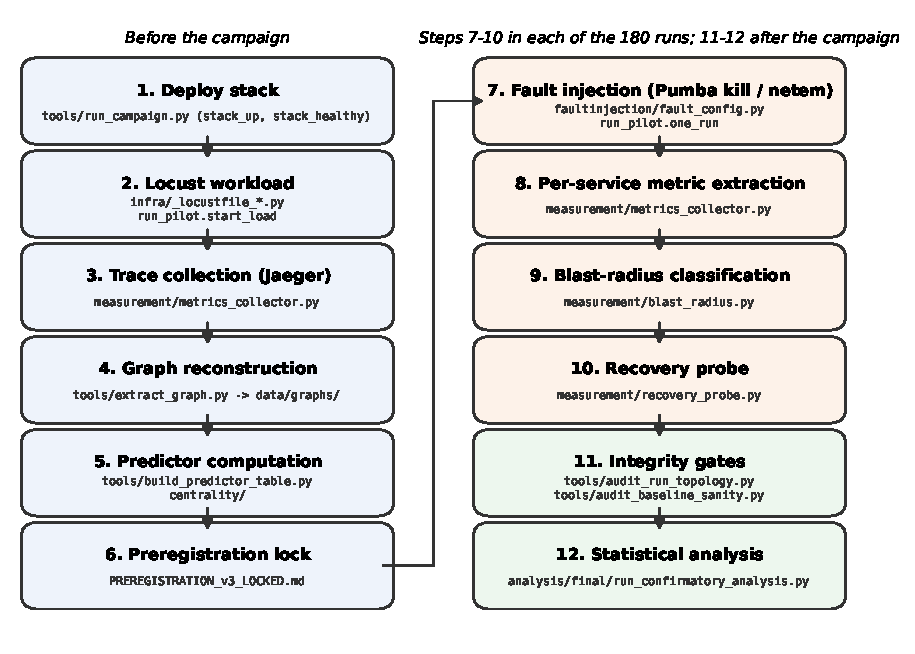
\includegraphics[width=\columnwidth]{generated/figures/fig_pipeline.pdf}
\caption{Pipeline in execution order. Each box names the repository files that carry out the
step; the steps from fault injection to the recovery probe repeat in every run.}
\label{fig:pipeline}
\end{figure}

\subsection{Testbed}
\label{sec:testbed}

All experiments ran on one host, configured as in Table~\ref{tab:tbl_ieee_testbed}. The
application stacks, Jaeger and Pumba ran as containers inside the virtual machine of Docker
Desktop's WSL2 backend, while the load generator and the campaign runner ran as host processes
(Fig.~\ref{fig:deployment}). The runner stops every stack before the campaign and brings up one
application at a time, so the two never shared the \val{testbed_docker_vm_gib}~GiB memory
ceiling of the virtual machine. The Social Network stack has \val{testbed_containers_sn}
containers and the Hotel Reservation stack \val{testbed_containers_hr}. Traces were collected
with Jaeger \val{version_jaeger}, one all-in-one instance per application with
\val{testbed_jaeger_storage} storage. The memory ceiling, host memory and container counts were
recorded on \val{testbed_vm_record_date}, before the campaign. The host operating system, CPU
and Docker Desktop version were queried on \val{testbed_measured_on}, after the campaign, and
Table~\ref{tab:tbl_ieee_testbed} marks them as measured.

\begin{table*}[!t]
\centering
\caption{Testbed and run protocol; host values marked as measured were queried after the campaign}
\label{tab:tbl_ieee_testbed}
\footnotesize
\setlength{\tabcolsep}{3pt}

\begin{tabular}{p{3.3cm}p{9.6cm}p{4.6cm}}
\toprule
\textbf{Item} & \textbf{Value} & \textbf{Source} \\
\midrule
Host OS & Microsoft Windows 11 Home Single Language (10.0.26300) & measured on 2026-10-20 \\
Host CPU & 12th Gen Intel(R) Core(TM) i7-1255U, 10 cores, 12 threads & measured on 2026-10-20 \\
Host RAM (GB) & 15.7 & recorded 2026-09-24 \\
Docker Desktop & 4.91.0, WSL2 backend & version measured on 2026-10-20 \\
Docker VM memory (GiB) & 7.598 (WSL2 default) & recorded 2026-09-24 \\
Docker client / Compose & 29.8.0 / 5.5.1 & client recorded 2026-10-18; Compose measured on 2026-10-20 \\
Containers per stack & Social Network 27, Hotel Reservation 24 & recorded 2026-09-24; one stack at a time \\
DeathStarBench commit & 6ecb097 & pinned upstream commit \\
Jaeger & 1.62.0 all-in-one, in-memory storage & compose override file \\
Pumba & ghcr.io/alexei-led/pumba, untagged image & version not recorded \\
Python & 3.13.2 & repository README \\
Python libraries & NumPy 2.1.2, pandas 2.2.3, SciPy 1.14.1, statsmodels 0.14.6, NetworkX 3.6.1, matplotlib 3.9.2 & repository README \\
Locust & 2.46.3; 25 users, spawn rate 10 users/s, 0.5 to 1.5 s between requests & runner and Locust files \\
Request mix, Social Network & compose post 3, home timeline 5, user timeline 2 & Locust task weights \\
Request mix, Hotel Reservation & search 6, reservation 2, user 2, recommendation 1 & Locust task weights \\
Load before the fault (s) & 60, also the baseline window & runner \\
Fault hold (s) & 30 & runner \\
Recovery probe (s) & poll 1, confirmation 5, lag 5, cap 180 & runner \\
Cooldown (s) & 20 & runner \\
\bottomrule
\end{tabular}
\end{table*}


\begin{figure}[!t]
\centering
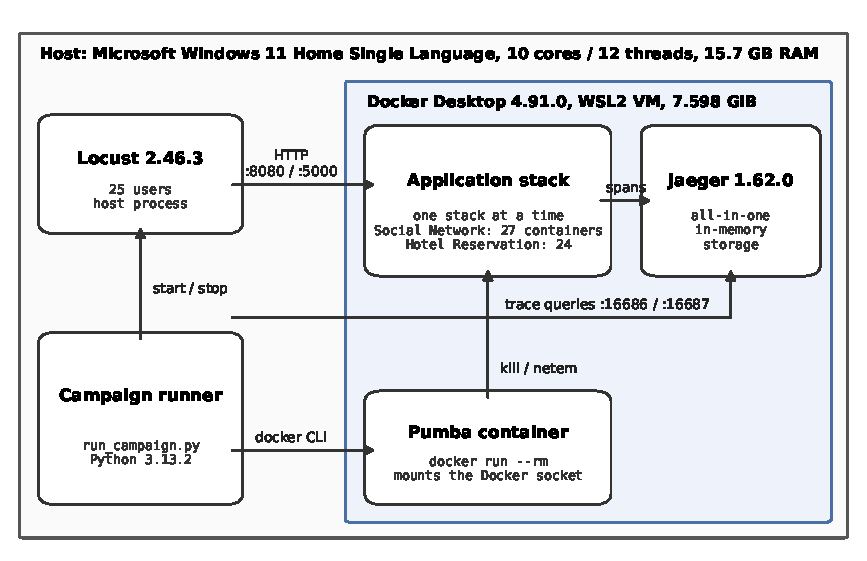
\includegraphics[width=\columnwidth]{generated/figures/fig_deployment.pdf}
\caption{Testbed deployment: the host, the Docker Desktop virtual machine with the application
stack, Jaeger and Pumba containers, and the Locust load generator and campaign runner on the
host.}
\label{fig:deployment}
\end{figure}

\subsection{Applications and Dependency Graphs}
\label{sec:apps}

Both applications come from DeathStarBench \cite{gan2019}, built from one pinned upstream
commit, \val{dsb_commit}, so the code under test was identical in every run. Their shapes
differ. Social Network is deep and fans out from a single composition service, while Hotel
Reservation is shallow and close to a star around its gateway. That difference turned out to
decide what each application could show (Section~\ref{sec:res-h1}).

The dependency graphs were taken from traces and not from documentation, because a diagram
shows the calls a system can make while the hypotheses concern the calls it makes under the
workload being perturbed. A directed edge runs from caller to callee wherever a span of one
service is the parent of a span of another \cite{sigelman2010}. The Social Network graph came
from \val{graph_sn_traces_examined} traces holding \val{graph_sn_spans_examined} spans, and
the Hotel Reservation graph from \val{graph_hr_traces_examined} traces holding
\val{graph_hr_spans_examined} spans. The graphs have \val{graph_sn_nodes} and
\val{graph_hr_nodes} services, with \val{graph_sn_edges} and \val{graph_hr_edges} observed call
edges (Figs.~\ref{fig:graph-sn} and~\ref{fig:graph-hr}). Both were frozen as files, and every
predictor is computed from those files.

\begin{figure}[!t]
\centering
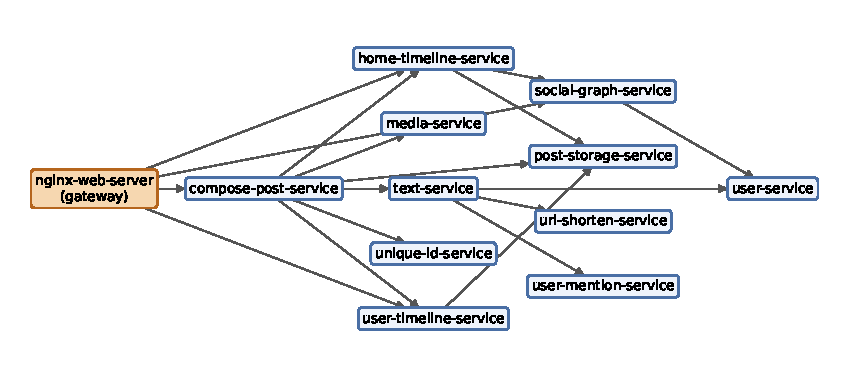
\includegraphics[width=\columnwidth]{generated/figures/fig_graph_sn.pdf}
\caption{Social Network dependency graph as observed in traces, with the gateway marked.}
\label{fig:graph-sn}
\end{figure}

\begin{figure}[!t]
\centering
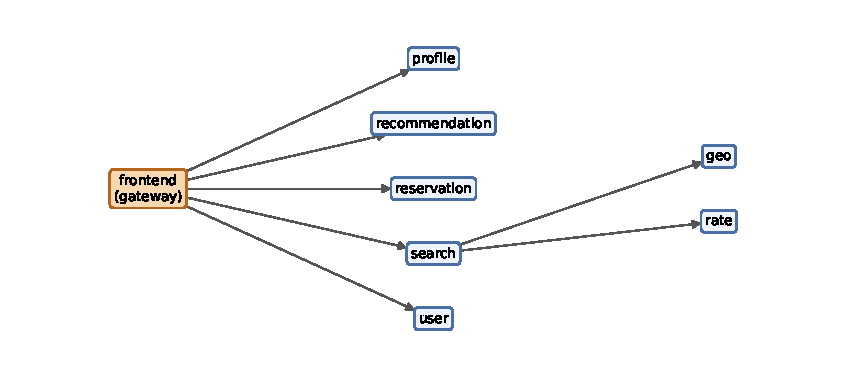
\includegraphics[width=\columnwidth]{generated/figures/fig_graph_hr.pdf}
\caption{Hotel Reservation dependency graph as observed in traces, with the gateway marked.}
\label{fig:graph-hr}
\end{figure}

The observed Hotel Reservation graph differs from the documented one. Of the
\val{hr_manifest_expected_edges} call edges implied by the published service tree, the traces
recover \val{hr_manifest_edges_recovered}. Two never appear under this workload,
%[id:hr_manifest_edges_missed]
\val{hr_manifest_edges_missed_names}, and one edge the tree does not list appears,
\val{hr_manifest_edges_extra}, which seems to stand in for the missing search-to-profile call.
The difference matters for one service: user has a single observed caller,
%[id:hr_user_observed_caller_count]
\val{hr_user_observed_callers}, where the documentation implies two. The observed graph is
used, and the divergence is reported.

\subsection{Analysis Set}
\label{sec:analysis-set}

Every correlation excludes the one service per application that has no caller in the graph:
nginx-web-server in Social Network and frontend in Hotel Reservation. A gateway receives
traffic only from the load generator, which is not a node of the graph, so its ancestor count
is zero by construction. Killing it also removes the only entry to the application and leaves
the outcome undefined. Without the gateways, \val{sn_services} services remain in Social
Network and \val{hr_services} in Hotel Reservation.

\subsection{Predictors}
\label{sec:predictors}

Section~\ref{sec:problem} defines the caller count and the hybrid metric. The ten further
comparators are degree, in-degree, out-degree, betweenness, closeness, eigenvector centrality
\cite{bonacich1987}, PageRank \cite{brin1998}, a composite rank, descendant count and dominator
subtree size, the number of services reachable from the gateway only through a given service.
Dominators are a classical notion for flow graphs \cite{lengauer1979}; here they are computed
with the immediate-dominator routine of NetworkX. Centralities follow the standard definitions
\cite{freeman1978}, and betweenness uses the algorithm of Brandes \cite{brandes2001}. The plan
forbade dropping any comparator after results were seen, and none was dropped.

The hybrid metric's weight values, \val{hybrid_w_in}, \val{hybrid_w_out} and
\val{hybrid_w_btw}, come from the project's original proposal, where an empirical search had
chosen them, so they were not fixed independently of all data. The locked plan called for tuning the weights on Social Network and
freezing them for Hotel Reservation. That step was never run (Deviation 10), and no weights were
re-tuned on campaign data. %[id:hybrid_weights_lockfile_exists] %[id:hybrid_weights_reoptimised_on_campaign]
A sensitivity analysis over every weighting on the preregistered grid, run after the
confirmatory results were known, is reported in Section~\ref{sec:res-weights}.
%[id:hybrid_weights_grid_evaluated_post_hoc]

Two predictor-application pairs were declared degenerate in advance because the predictor is
constant across the analysis set, which leaves Spearman's $\rho$ undefined. Eigenvector
centrality is zero for every analysed Social Network service, %[id:degenerate_sn_value]
since the reconstructed graph is acyclic, and every Hotel Reservation service has exactly one
direct caller, so in-degree is constant there. Both pairs are left out of the test family,
because a degenerate graph property is not a null result and counting it as one would dilute
the correction. That leaves \val{testable_pairs} testable pairs of the
\val{total_predictor_pairs} considered.

\subsection{Workload and Run Protocol}
\label{sec:protocol}

Each run starts the load generator, Locust \val{version_locust}, with
\val{protocol_load_users} users spawned at \val{protocol_spawn_rate} per second. Each simulated
user waits between \val{protocol_sn_wait_min_s} and \val{protocol_sn_wait_max_s} seconds
between requests %[id:protocol_hr_wait_min_s] %[id:protocol_hr_wait_max_s]
and draws each request from a fixed weighted mix (Table~\ref{tab:tbl_ieee_testbed}). On
Social Network the weights are \val{protocol_sn_task_weight_compose_post} for composing a post,
\val{protocol_sn_task_weight_read_home_timeline} for reading a home timeline and
\val{protocol_sn_task_weight_read_user_timeline} for reading a user timeline. On Hotel
Reservation they are \val{protocol_hr_task_weight_hotel_search} for a hotel search,
\val{protocol_hr_task_weight_make_reservation} for a reservation,
\val{protocol_hr_task_weight_get_user} for a user lookup and
\val{protocol_hr_task_weight_get_recommendations} for recommendations.

The load runs for \val{protocol_warmup_s} seconds before the fault, and the fault-free baseline
percentiles are computed over that same \val{protocol_baseline_window_s}-second window. The
window therefore opens when the load generator starts and includes its ramp-up (Deviation 13);
its length was the same in every run. %[id:protocol_baseline_window_distinct]
The fault is then held for \val{protocol_fault_duration_s} seconds, the recovery probe runs,
and a \val{protocol_cooldown_s}-second cooldown separates one run from the next.

Faults are injected with Pumba, which the runner starts as a short-lived container that acts on
the target container through the Docker socket; every command goes through the Docker
\val{version_docker_client} client. Table~\ref{tab:tbl_ieee_commands} lists the command lines,
generated from the runner code. A kill fault sends \val{fault_kill_signal}, which ends the
process without draining connections or answering requests in flight. A latency fault applies
a \texttt{tc netem} rule that adds \val{fault_latency_delay_ms}~ms of delay, with
\val{fault_latency_jitter_ms}~ms of jitter, to the container's network interface. The kill asks
what happens when a dependency vanishes; the delay asks what happens when it stays up but
answers late.

\begin{table*}[!t]
\centering
\caption{Command lines issued in each run, generated from the runner code}
\label{tab:tbl_ieee_commands}
\footnotesize
\setlength{\tabcolsep}{3pt}

\begin{tabular}{p{2.9cm}p{11.9cm}p{2.7cm}}
\toprule
\textbf{Step} & \textbf{Command} & \textbf{Source} \\
\midrule
Start the load & \texttt{python -m locust -f <locustfile> -{}-host <url> -{}-headless -{}-users <users> -{}-spawn-rate 10 -{}-run-time <duration>s -{}-only-summary -{}-loglevel ERROR} & runner, load start \\
Find the target container & \texttt{docker ps -{}-filter label=com.docker.compose.service=<service> -{}-format '\{\{.Names\}\}\textbackslash\{\}t\{\{.Label "com.docker.compose.service"\}\}'} & runner, target resolution \\
Kill fault & \texttt{docker run -{}-rm -v /var/run/docker.sock:/var/run/docker.sock ghcr.io/alexei-led/pumba kill -{}-signal SIGKILL <container>} & fault configuration \\
Latency fault & \texttt{docker run -{}-rm -v /var/run/docker.sock:/var/run/docker.sock ghcr.io/alexei-led/pumba netem -{}-duration 30s delay -{}-time 500 -{}-jitter 100 <container>} & fault configuration \\
Restore after a kill & \texttt{docker compose up -d <service>} & runner, restore \\
Clean up after a latency fault & \texttt{docker compose up -d -{}-force-recreate <service>} & runner, clean-up \\
\bottomrule
\end{tabular}
\end{table*}


The runner finds the target as the one container whose \texttt{com.docker.compose.service}
label equals the service name exactly, and it stops if none or several match, so that a fault
cannot land on a different service from the one recorded (Deviation 2). Timing differs by fault
type. A kill completes at once; the runner waits out the fault window, restores the service
with \texttt{docker compose up -d}, and takes the fault-removal instant when that command
returns. Because \texttt{pumba netem} blocks for its declared duration, the runner launches it
as a separate process and takes the fault-removal instant when that process exits. After the
recovery probe of every latency run, the runner recreates the target container so that no
residual netem rule reaches the next run (Deviation 4). Algorithm~\ref{alg:run} gives one run in
full, with warm-up and baseline window $W$ of \val{protocol_warmup_s}~s, fault hold $H$ of
\val{protocol_fault_duration_s}~s, probe interval $P$ of \val{trec_poll_interval_nominal_s}~s,
confirmation period $K$ of \val{protocol_confirm_s}~s, probe lag $L$ of
\val{protocol_probe_lag_s}~s and recovery cap $C$ of \val{protocol_recovery_cap_s}~s.

\begin{algorithm}[!t]
\caption{One campaign run (\texttt{one\_run} in \texttt{tools/run\_pilot.py}), called in
manifest order with a cooldown after each run}
\label{alg:run}
\begin{algorithmic}[1]
\Require application $a$, service $s$, fault type $f$, repetition $r$, graph $G$ of $a$
\State $c \gets$ the running container whose label \texttt{com.docker.compose.service}
equals the compose name of $s$; stop unless exactly one matches
\State start the Locust load against the gateway of $a$
\State wait $W$; $B \gets$ per-service baseline percentiles and error rates over the last $W$
\State $t_{\mathrm{inj}} \gets$ now; issue the Pumba command for $f$ on $c$
\Comment{kill: synchronous; latency: background process}
\State wait $H$; $t_{\mathrm{end}} \gets$ now
\State $D \gets$ services degraded in $[t_{\mathrm{inj}}, t_{\mathrm{end}}]$ relative to $B$
\State persist the raw spans of the baseline and fault windows
\If{$f = \text{kill}$}
  \State run \texttt{docker compose up -d} for $s$
\Else
  \State wait for the Pumba process to exit
\EndIf
\State $t_{\mathrm{rm}} \gets$ now \Comment{fault-removal instant}
\State $\Trec \gets$ recovery probe from $t_{\mathrm{rm}}$ with interval $P$, confirmation $K$,
lag $L$ and cap $C$
\If{$f \neq \text{kill}$}
  \State run \texttt{docker compose up -d -{}-force-recreate} for $s$
\EndIf
\State classify $D$ into ancestors, descendants and unrelated services of $s$ in $G$
\State stop the load; \Return the run record
\end{algorithmic}
\end{algorithm}

The design is fully crossed and balanced. Each analysable service receives each fault type
\val{campaign_reps_per_cell} times, giving \val{campaign_cells} cells and
\val{campaign_runs_total} runs, \val{sn_runs} on Social Network and \val{hr_runs} on Hotel
Reservation. A run with incomplete telemetry is discarded and repeated in its own cell; it is
never replaced elsewhere and never analysed as zeros. The same rule covered the
\val{deviations_runs_invalidated} runs invalidated by Deviations 1, 2 and 4, which were
collected again in their cells. %[id:deviation_1_runs_invalidated] %[id:deviation_2_runs_invalidated] %[id:deviation_4_runs_invalidated]
The campaign ran from \val{campaign_start_utc} to \val{campaign_end_utc} UTC, measured from the
first to the last end-timestamp of the kept runs, and lost \val{campaign_runs_failed} runs to
telemetry failure. The raw spans of the baseline and fault windows were stored for every run,
so any later change to a metric definition can be replayed on the original data without
repeating the experiment.

\subsection{Per-Service Latency and Error Attribution}
\label{sec:attribution}

The latency definition needed more care than any other part of the method, because the obvious
implementation is wrong in a way that is easy to miss. A tracing backend asked for the traces
involving a service returns every trace in which the service appears, and the root span of each
trace times the whole request from end to end. A percentile over those root spans, labelled as
the p95 of the service, is really the end-to-end p95 of every request that passed through it,
and every service on a request path receives the same value. Error rate has the same flaw if a
trace counts as failed whenever any of its spans carries an error. Services on a shared path
then become indistinguishable, and a threshold flags them as a group.

Fig.~\ref{fig:q3} shows the effect on Hotel Reservation under a latency fault in the search
service, using \val{q3_pilot_runs} pilot validation runs that are not part of the campaign.
Under the end-to-end scope, three services, %[id:q3_identical_baseline_services]
\val{q3_identical_baseline_names}, share an identical baseline p95 in both runs, and a
multiplicative threshold flags five services that were not faulted.
%[fig:fig_q3_artifact]
Two of them, profile and reservation, are neither ancestors nor descendants of search; they
share a trace with it and nothing more.

\begin{figure*}[!t]
\centering
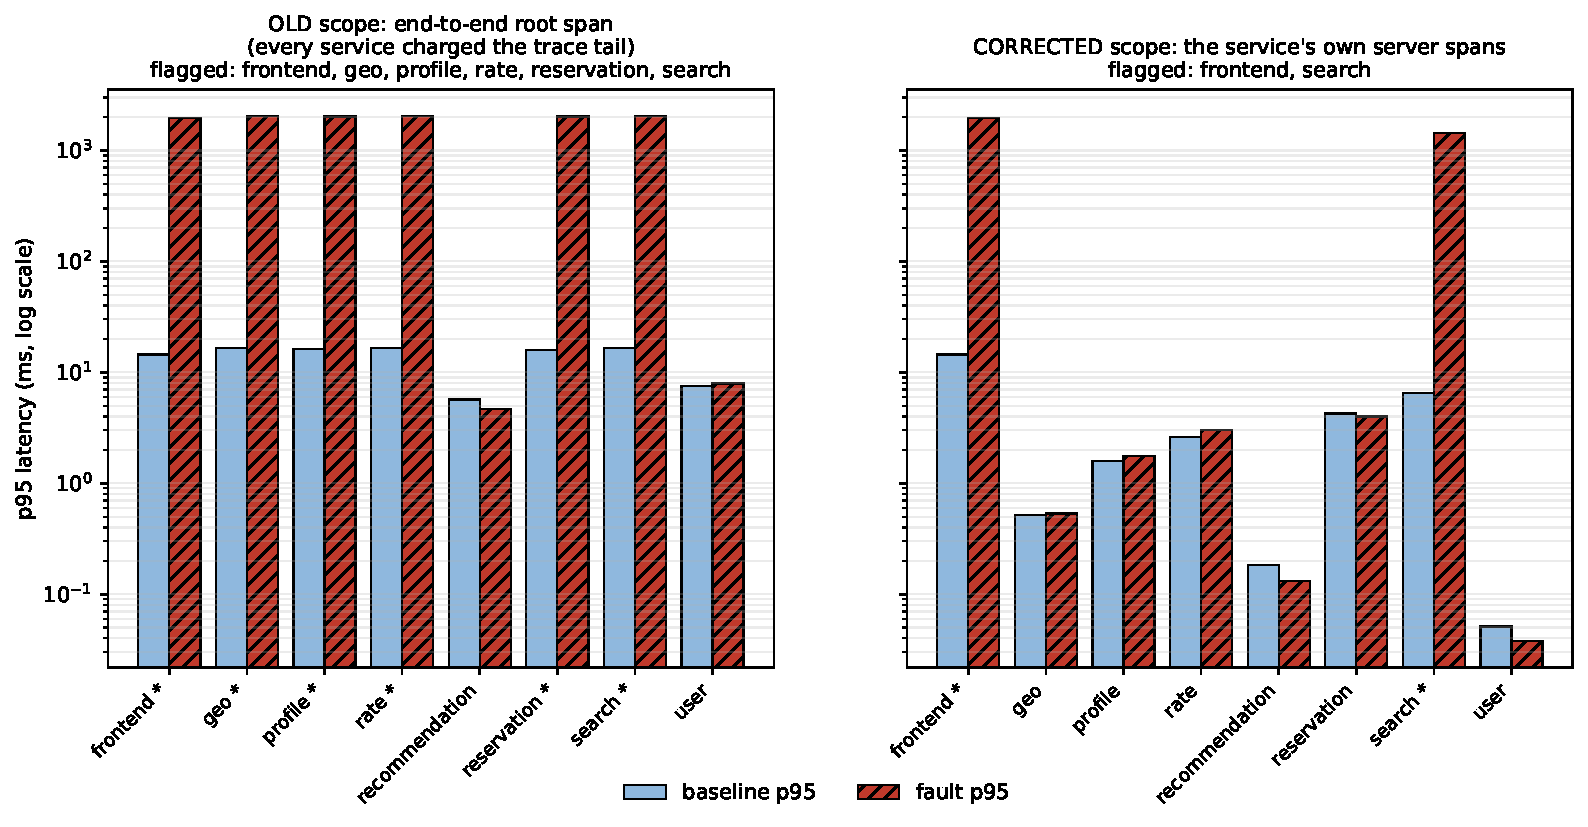
\includegraphics[width=0.82\textwidth]{generated/figures/fig_q3_artifact.pdf}
\caption{Per-service p95 on Hotel Reservation under a latency fault in search, measured on the
end-to-end root span of each trace (left) and on each service's own spans (right). An asterisk
marks a service flagged as degraded.}
\label{fig:q3}
\end{figure*}

Each service's latency is therefore measured on the spans that service emits itself. On Hotel
Reservation, whose spans carry a span-kind tag, client spans are excluded, because a client
span recorded by a service times its callee and would pass a downstream delay back up. Social
Network's spans carry no span-kind tag, so all of a service's spans were used there, and
\val{sn_spans_selected_client_pct}\% of the spans used were client spans. A post hoc replay
restricted to server spans changed the outcome of \val{replay_runs_changed} of \val{replay_runs}
runs and none of the service-level medians, and the primary result came out identical
(Deviation 11). %[id:replay_service_medians_changed] %[id:replay_primary_identical] %[id:sn_span_samples_fallback]
An error counts against a service only when one of its own spans is tagged as an error, divided
by the number of traces in which the service appears. With per-service attribution, the same
two pilot runs flag one non-faulted service instead of five, and that service is an ancestor of
search. %[fig:fig_q3_artifact]
The services that drop out keep a flat service time while the end-to-end value charged to them
grows more than a hundredfold, the signature of a measurement artifact; shared-resource
contention would raise their own service times.

\subsection{Outcomes: Blast Radius and Recovery Time}
\label{sec:outcomes}

A service counts as degraded when either of two conditions holds on its own spans during the
fault window. The latency condition requires its p95 to exceed
\val{threshold_degradation_factor}$\times$ its baseline p95 and to rise by at least
\val{threshold_degradation_floor_ms}~ms. The error condition requires its error rate to rise by
at least \val{threshold_error_rate_abs} in absolute terms. The absolute floor became necessary
once percentiles were truly per service: some services here have baseline p95 values in the
hundredths of a millisecond, where a purely multiplicative rule reacts to scheduler noise
(Deviation 1). Both conditions are evaluated at full precision. Degraded services are split
into the ancestor, descendant and unrelated counts of Section~\ref{sec:problem}.

Which indicator carries the signal depends on the fault type, and the plan fixed the pairing in
advance. Under kill faults the primary indicator is error rate, because requests fail; in the
pilot the sign of the kill-fault change in p95 even differed between the two applications, so
it is never pooled. Under latency faults the change in p95 is the primary indicator and error
rate carries no signal, because nothing has failed.

Recovery time, \Trec, is the number of seconds from fault removal until the changes in p95, p99,
error rate and downstream-affected count are all back within
\val{protocol_recovery_tolerance_pct}\% of their baseline and stay
there for a \val{protocol_confirm_s}-second confirmation period. Timing from removal matters,
since timing from injection would include the whole fault and could never fall below it. The
probe polls at a nominal \val{trec_poll_interval_nominal_s}-second interval, with an effective
resolution of \val{trec_poll_interval_eff_min_s} to \val{trec_poll_interval_eff_max_s} seconds
measured as the median gap between samples within each run. Each sample reads a window lagged
\val{protocol_probe_lag_s} seconds into the past, because tracing backends flush spans in
batches, and needs at least \val{protocol_min_traces} traces before its percentiles can vote for
recovery. A run that has not recovered within \val{protocol_recovery_cap_s} seconds is recorded
as right-censored and never filled in with a number. No run was censored.
%[id:campaign_runs_censored]
Observed recovery times ranged from \val{trec_min_s}~s to \val{trec_max_s}~s, with a median of
\val{trec_median_s}~s. The plan stated in advance that a low censoring rate would make the rank
test the primary test for \Trec, with survival models reported beside it; at a censoring rate of
\val{campaign_censoring_rate_pct}\%, that rule applied (Deviation 6).

\subsection{Statistical Analysis}
\label{sec:stats}

Associations between a graph predictor and a measured outcome are tested with Spearman's
$\rho$ at the service level, after taking the median over each service's repetitions; the
repetitions make each service's value more precise but add no points to the correlation.
Significance comes from permutation tests, exact where all orderings can be enumerated and
otherwise from \val{primary_n_permutations} random permutations, with one added to both counts
so that no p-value is zero \cite{phipson2010}. The asymptotic approximation is unreliable at
these sample sizes and with the ties these graphs produce. Confidence intervals are
bias-corrected and accelerated bootstrap intervals \cite{efron1987}, with a percentile interval,
marked as such, where ties leave the bias correction undefined. For recovery time the Cox
proportional hazards model \cite{cox1972} and the log-rank test serve as secondary analyses. The
analysis ran on Python \val{version_python}, with SciPy \val{version_scipy} supplying ranks and
the reference Spearman implementation and statsmodels \val{version_statsmodels} the survival
models.

Tests fall into three families, each corrected separately with the Benjamini-Hochberg
procedure at $q = \val{fdr_q}$ \cite{benjamini1995}. The confirmatory family holds
\val{conf_family_size} tests on kill faults: the \val{testable_pairs} testable pairs, each
against $Y$ and against \Trec. The replication family repeats them on latency faults.
%[id:repl_family_size]
A third, exploratory family covers secondary outcomes and carries no confirmatory weight. The
plan considered pooling the families into one correction and rejected it, because the
confirmatory and replication families ask the same question under different faults. Two gates
run before any statistic: one confirms that every expected service was present in every run,
and the other compares each run's fault-free baseline with those of all other runs, using the
median and the median absolute deviation. All \val{integrity_checks_total} pre-analysis
integrity checks passed. %[id:integrity_checks_passed]

\subsection{Preregistration and Deviations}
\label{sec:deviations}

The plan was locked before the campaign started \cite{nosek2018}, and every later change was
logged with its date and with whether campaign data had been analysed by then.
\val{deviations_total} deviations were recorded; Appendix~\ref{app:deviations} lists them.
\val{deviations_no_data} invalidated no data. The other \val{deviations_with_data} invalidated
\val{deviations_runs_invalidated} runs, each collected again in its own cell, so the final
dataset is complete and balanced. Deviation 1 added the absolute latency floor after the
pre-launch rehearsal, Deviation 2 replaced a substring match that had faulted the wrong
container, and Deviation 4 dealt with a netem rule that outlived its run and inflated later
baselines. The remaining deviations concern the analysis or its reporting: the rank test
becoming primary for recovery time, an asymptotic p-value quoted in the plan, exact p-values
reported only as supplementary, the weight tuning that was not run, the Social Network span
selection, and Deviation 13, found while this paper was written, which records that the
baseline window includes the load ramp-up; it invalidated no run, and the baseline gate found no
anomalies.
